% sprawozdanie_projekt_udostępnianie_ekranu.tex
% Projekt indywidualny - system do udostępniania ekranu 
% Jordan Parviainen 2023

\documentclass[a4paper,11pt]{article}

% Packages
\usepackage[utf8]{inputenc}  		% Kodowanie pliku
\usepackage[T1]{fontenc}
\usepackage[T1]{polski}			% Język polski
\usepackage{graphicx}			% Grafika
\usepackage[inkscapeformat=pdf]{svg}	% .svg tylko w postaci wektorowej - nie png! .pdf/.eps/.ps/.png/.pdf_tex
\usepackage{listings}
\usepackage{float}
\usepackage{lmodern}
\usepackage{biblatex}
\usepackage{hyperref}

\lstdefinestyle{myStyle}{
    belowcaptionskip=1\baselineskip,
    breaklines=true,
    frame=none,
    numbers=none,
    basicstyle=\footnotesize\ttfamily,
    keywordstyle=\bfseries\color{green!40!black},
    commentstyle=\itshape\color{purple!40!black},
    identifierstyle=\color{blue},
    % backgroundcolor=\color{gray!10!white},
    extendedchars = true,  % Extended ASCII
    literate      =        % Support additional characters
      {á}{{\'a}}1  {é}{{\'e}}1  {í}{{\'i}}1 {ó}{{\'o}}1  {ú}{{\'u}}1
      {Á}{{\'A}}1  {É}{{\'E}}1  {Í}{{\'I}}1 {Ó}{{\'O}}1  {Ú}{{\'U}}1
      {à}{{\`a}}1  {è}{{\`e}}1  {ì}{{\`i}}1 {ò}{{\`o}}1  {ù}{{\`u}}1
      {À}{{\`A}}1  {È}{{\`E}}1  {Ì}{{\`I}}1 {Ò}{{\`O}}1  {Ù}{{\`U}}1
      {ä}{{\"a}}1  {ë}{{\"e}}1  {ï}{{\"i}}1 {ö}{{\"o}}1  {ü}{{\"u}}1
      {Ä}{{\"A}}1  {Ë}{{\"E}}1  {Ï}{{\"I}}1 {Ö}{{\"O}}1  {Ü}{{\"U}}1
      {â}{{\^a}}1  {ê}{{\^e}}1  {î}{{\^i}}1 {ô}{{\^o}}1  {û}{{\^u}}1
      {Â}{{\^A}}1  {Ê}{{\^E}}1  {Î}{{\^I}}1 {Ô}{{\^O}}1  {Û}{{\^U}}1
      {œ}{{\oe}}1  {Œ}{{\OE}}1  {æ}{{\ae}}1 {Æ}{{\AE}}1  {ß}{{\ss}}1
      {ẞ}{{\SS}}1  {ç}{{\c{c}}}1 {Ç}{{\c{C}}}1 {ø}{{\o}}1  {Ø}{{\O}}1
      {å}{{\aa}}1  {Å}{{\AA}}1  {ã}{{\~a}}1  {õ}{{\~o}}1 {Ã}{{\~A}}1
      {Õ}{{\~O}}1  {ñ}{{\~n}}1  {Ñ}{{\~N}}1  {¿}{{?`}}1  {¡}{{!`}}1
      {°}{{\textdegree}}1 {º}{{\textordmasculine}}1 {ª}{{\textordfeminine}}1
      {£}{{\pounds}}1  {©}{{\copyright}}1  {®}{{\textregistered}}1
      {«}{{\guillemotleft}}1  {»}{{\guillemotright}}1  {Ð}{{\DH}}1  {ð}{{\dh}}1
      {Ý}{{\'Y}}1    {ý}{{\'y}}1    {Þ}{{\TH}}1    {þ}{{\th}}1    {Ă}{{\u{A}}}1
      {ă}{{\u{a}}}1  {Ą}{{\k{A}}}1  {ą}{{\k{a}}}1  {Ć}{{\'C}}1    {ć}{{\'c}}1
      {Č}{{\v{C}}}1  {č}{{\v{c}}}1  {Ď}{{\v{D}}}1  {ď}{{\v{d}}}1  {Đ}{{\DJ}}1
      {đ}{{\dj}}1    {Ė}{{\.{E}}}1  {ė}{{\.{e}}}1  {Ę}{{\k{E}}}1  {ę}{{\k{e}}}1
      {Ě}{{\v{E}}}1  {ě}{{\v{e}}}1  {Ğ}{{\u{G}}}1  {ğ}{{\u{g}}}1  {Ĩ}{{\~I}}1
      {ĩ}{{\~\i}}1   {Į}{{\k{I}}}1  {į}{{\k{i}}}1  {İ}{{\.{I}}}1  {ı}{{\i}}1
      {Ĺ}{{\'L}}1    {ĺ}{{\'l}}1    {Ľ}{{\v{L}}}1  {ľ}{{\v{l}}}1  {Ł}{{\L{}}}1
      {ł}{{\l{}}}1   {Ń}{{\'N}}1    {ń}{{\'n}}1    {Ň}{{\v{N}}}1  {ň}{{\v{n}}}1
      {Ő}{{\H{O}}}1  {ő}{{\H{o}}}1  {Ŕ}{{\'{R}}}1  {ŕ}{{\'{r}}}1  {Ř}{{\v{R}}}1
      {ř}{{\v{r}}}1  {Ś}{{\'S}}1    {ś}{{\'s}}1    {Ş}{{\c{S}}}1  {ş}{{\c{s}}}1
      {Š}{{\v{S}}}1  {š}{{\v{s}}}1  {Ť}{{\v{T}}}1  {ť}{{\v{t}}}1  {Ũ}{{\~U}}1
      {ũ}{{\~u}}1    {Ū}{{\={U}}}1  {ū}{{\={u}}}1  {Ů}{{\r{U}}}1  {ů}{{\r{u}}}1
      {Ű}{{\H{U}}}1  {ű}{{\H{u}}}1  {Ų}{{\k{U}}}1  {ų}{{\k{u}}}1  {Ź}{{\'Z}}1
      {ź}{{\'z}}1    {Ż}{{\.Z}}1    {ż}{{\.z}}1    {Ž}{{\v{Z}}}1
}
\lstset{style=myStyle}

% Settings
\hoffset=-3.0cm                         % Mniejszy lewy margines
\textwidth=18cm                         % szerzej
\evensidemargin=0pt

\voffset=-3cm                           % Mniejszy górny margines
\textheight=27cm                        % szerzej wzdłuż
\frenchspacing                          % Bez spacji na końcu zdania.
\setlength{\parindent}{0pt}             % No paragraph indentation
\setlength{\parskip}{\medskipamount}    % Space between paragraphs
\raggedbottom                           % bez rozciagania strony


% Dodatkowe komendy
\newcommand\BS{\char`\\}                % \BS == back-slash
\newcommand\TY{\raise.17ex\hbox{$\scriptstyle\mathtt{\sim}$}}   % \TY == większa tylda w \tt
\setlength{\abovecaptionskip}{15pt plus 3pt minus 2pt}
\setlength{\belowcaptionskip}{15pt plus 3pt minus 2pt}

\title{%
    \huge{Sprawozdanie z projektu indywidualnego \\
    \ \\
    Temat: Wdrożenie prostego systemu do udostępniania ekranu komputera w sieci lokalnej}}
\author{\large{Autor projektu: Jordan Parviainen} \\ Opiekun projektu: mgr inż. Andrzej Toboła}
\begin{document}
    \maketitle
    \thispagestyle{empty}
    \begin{figure}[H]
        \centering
        
\includegraphics[width=0.7\textwidth]{PW-uroczysty-grafitowe.png}
    \end{figure}
    \begin{center}\huge{Wydział Elektryczny} \\
    \huge{Informatyka Stosowana} 
    \end{center}
    \newpage
    \thispagestyle{empty}
    \tableofcontents
    \newpage
    \pagenumbering{arabic}
    \section{Postawienie problemu i zadania}
        \subsection{Potrzeba}
        W dobie powszechnej informatyzacji i pracy zdalnej, coraz więcej rzeczy jest wykonywanych przy pomocy komputera. Rośnie wraz z tym potrzeba sprawnej współpracy pomiędzy użytkownikami.  
        Bardzo przydatna jest możliwość pokazania jak wykonać daną czynność poprzez udostępnienie obrazu swojego komputera, czy to na żywo, czy to nagrywając materiał wideo. 
        Z takimi potrzebami spotyka się także na uczelni, np. podczas zajęć laboratoryjnych z wykorzystaniem komputerów, gdzie często prowadzący pokazuje jak wykonać daną czynność, a studenci obserwują.
        Do tego celu wykorzystuje się często rzutniki, jednak nie jest to zawsze rozwiązanie wygodne czy optymalne. Bywają problemy z widocznością obrazu, a także nie każda sala jest do tego przystosowana.  
        \subsection{Pomysł na rozwiązanie}
        Aby znaleźć alternatywny sposób na rozwiązanie tego problemu, zamiast patrzeć w stronę sprzętu, można zwrócić uwagę na oprogramowanie. Czy nie byłoby łatwiej, gdyby studenci mogli oglądać ekran prowadzącego na swoich komputerach?
        Istnieją oczywiście już tego typu rozwiązania, powszechnie stosowane w pracy zdalnej, np. MSTeams, Zoom. Jednakże są to rozwiązania zbyt rozbudowane, a także nie zawsze dostępne. Nie są one dobrym środkiem 
        w przypadku np. zajęć laboratoryjnych, gdzie trzeba na szybko jedynie pokazać ekran. Perspektywa instalowania ciężkiego oprogramowanie i tworzenia wideokonferencji, dodawania użytkowników etc. jest odstraszająca.
        Dlatego też powstał pomysł stworzenia prostego systemu udostępniania obrazu ekranu komputera, który idealnie nie wymagałby instalacji oprogramowania klienckiego, ani długiej konfiguracji. 
    \section{Przegląd istniejących rozwiązań}
        \subsection{Programy do wideokonferencji}
        Jak już było wspomniane, istnieje wiele programów do wideokonferencji, które w ramach swojej funkcjonalności oferują udostępnianie ekranu. Są to np. MSTeams, Zoom, Google Meet, Skype, etc.
        Jednak w zastosowaniu do udostępniania obrazu ad-hoc np. w sieci lokalnej w laboratorium mają liczne wady, takie jak:
        \begin{itemize}
            \item Konieczność logowania/zakładania konta
            \item Konieczność instalowania oprogramowania klienckiego, często niemałego w rozmiarach. Co prawda istnieją wersje przeglądarkowe, ale bywają okrojone w funkcjonalności i nie działają optymalnie. 
            \item Problemy z jakością/obciążeniem sieci. W przypadku, gdy trzeba udostępnić obraz wielu użytkownikom w jednej sali, wysoce nieoptymalnym jest korzystanie z oprogramowania, którego strumieniowanie
            odbywa się za pośrednictwem zewnętrznego serwera.   
        \end{itemize}     
        \subsection{Programy typu zdalny pulpit}
        Dostępne są na rynku programy o funkcjonalności pozwalającej na kontrolę nad zdalnym komputerem. 
        Są to m.in. takie programy jak: TightVNC, TeamViewer, Windows Remote Desktop, CoScreen, Anydesk. 
        Rozwiązania te dzielą wady wymienione, powyżej, a ponadto potrafią być zbyt skomplikowane do użytku, jeśli potrzebne jest tylko udostępnianie ekranu. 
        Ponadto często są to rozwiązania komercyjne, o zamkniętym kodzie źródłowym i płatnej licencji. 
        W laboratorium Sieci Komputerowych użyte było rozwiązanie oparte na skrypcie uruchamiającym i koordynującym połączenie za pomocą TightVNC. 
        Niestety, oznaczało to konieczność instalacji TightVNC na każdym komputerze, a samo udostępnianie np. okna terminala obwarowane było ograniczeniami i koniecznością ręcznego ustawiania np. rozdzielczości. 
    \section{Opis rozwiązania}
        \subsection{Pomysł}
        Nadzieję w tym projekcie położono w nowoczesnej przeglądarkowej technologii WebRTC. Pozwala ona na strumieniowanie obrazu i dźwięku przez przeglądarkę internetową w topologii punkt-do-punktu. 
        Jest to kompleksowe rozwiązanie obejmujące kompresję, kodowanie, szyfrowanie strumienia i wykorzystanie akceleracji sprzętowej.
        Ponadto technologia zawiera też mechanizmy zapewniające stałe bezpośrednie połączenie pomiędzy użytkownikami, nawet w skomplikowanych konfiguracjach sieciowych z NAT-ami.
        Cała ta moc jest udostępniona przez JavaScript-owe API w każdej popularnej przeglądarce internetowej (silniki Chromium i Gecko), oprócz tych opartych na silniku WebKit w produktach Apple. 
        \subsection{Poszukiwanie gotowych rozwiązań}
        Możnaby pokusić się o samodzielne napisanie rozwiązania, jednak lepiej było najpierw przeszukać zasoby gotowych rozwiązań o otwartym kodzie źródłowym,
        czy przypadkiem jakaś część tego, co jest potrzebne nie została już przez kogoś wykonana.
        Rozpoczęto swoje poszukiwania na najpopularniejszej stronie do udostępniania kodu - \emph{github.com}. Dosyć szybko znalazło się coś nadającego się.
        \subsection{Znalezione oprogramowanie}
        Znaleziony zostało publicznie dostępny kod aplikacji internetowej wykorzystującej technologię WebRTC do udostępniania ekranu z poziomu przeglądarki.
        Aplikacja \cite{2} nosi nazwę Laplace i jest autorstwa Adama Jordana.
        Jest to prosty serwer HTTP napisany w języku Go. 
        Serwuje on pliki części frontendowej i komunikuje się z nią za pomocą protokołu WebSocket w celu negocjacji połączenia WebRTC (signaling). 
        Część kliencka (przeglądarkowa) aplikacji napisana jest w czystym Javascript. Cała aplikacja ma niewiele funkcjonalności, ale za to kod jest zwięzły i całość ma niewielki rozmiar.
        \subsection{Działanie aplikacji}
        Działanie aplikacji polega na tym, że gdy ktoś chce udostępnić innym swój ekran, wybiera odpowiednią opcję i tworzy tzw. "pokój", 
        który ma przypisany identyfikator i do którego mogą dołączyć inni używając tego identyfikatora. 
        Zgodnie ze specyfikacją WebRTC, serwer nie pośredniczy w strumieniowaniu obrazu, a jedynie w nawiązaniu połączenia i jego utrzymaniu między użytkownikami.   
        Maszyna osoby udostępniającej ekran wysyła pakiety transmisji do każdej maszyny oglądającego. 
        Poniżej znajduje się schemat przedstawiający architekturę i działanie aplikacji: 
        \begin{figure}[H]
        \centering
        \def\svgwidth{\columnwidth}
        \includesvg[width=1\textwidth]{proj-arch}
        \caption{Schemat architektury sieciowej aplikacji}
        \label{rys1:label}
        \end{figure}
        \subsection{Więcej o WebRTC}
        Nawiązywanie połączenia punkt-do-punktu zaczyna się od zgłoszenia się maszyny chcącej nawiązać połączenie do serwera sygnalizacyjnego(ang. \emph{signaling server}).
        Następnie, serwer sygnalizacyjny ustala parametry połączenia nowej maszyny do pozostałych, korzystając z technologii ICE - (ang.\emph{Interactive Connectivity Establishment}).
        Jest to protokół służący do znajdowania sposobu, w jaki komputery mogą być ze sobą połączone jak najbardziej bezpośrednio, jak to jest możliwe. 
        Wykrywa możliwości obchodzenia m.in. NAT-ów i firewall-i. 
        W tym procesie znajdowani są tzw. kandydaci ścieżek i adresów połączeń uszeregowanych według skuteczności i informacja ta jest przesyłana do klientów, 
        którzy następnie nawiązują według tych informacji połączenia bezpośrednio z innymi klientami.  
    \section{Wdrożenie rozwiązania} 
        \subsection{Środowisko wdrożeniowe i cel}
        Celem projektu jest wdrożenie opisanego przeze mnie rozwiązania do laboratorium Sieci Komputerowych w gmachu Elektrycznym Politechniki Warszawskiej. 
        Nie jest to jedyny cel, idealnie byłoby przygotować prostą ścieżkę do zastosowania podobnego rozwiązania w innych, podobnych środowiskach.    
        Laboratorium Sieci Komputerowych składa się z kilkunastu maszyn połączonych w lokalną sieć o dużej przepustowości zarówno wewnętrznej, jak i do internetu.
        Na maszynach tych standardowo używany jest Arch Linux podnoszony z sieci, więc instalacja i konfiguracja była robiona z myślą o tym środowisku.  
        \subsection{Co było do zrealizowania}
        W ramach wdrożenia zrealizowano następujące rzeczy: 
        \begin{itemize}
            \item Dostosowano oprogramowanie do warunków sieci lokalnej i przygotowano jego repozytorium.
            \item Napisano skrypty instalacyjne pod system operacyjny Arch Linux.
            \item Napisano skrypty usprawniające pracę z oprogramowaniem do udostęniania ekranu.
        \end{itemize}
        \subsection{Modyfikacja oprogramowania}
        \begin{itemize}
            \item Dodano punkt końcowy do interfejsu REST serwera, zwracający identyfikator ostatnio utworzonego "pokoju", co umożliwia automatyzację otwierania ekranu udostępnianego przez prowadzącego w laboratorium.  
            \item Dodano możliwość przekazania w fazie kompilacji zmiennej z lokalizacją plików statycznych serwera HTTP.
            \item Ustawiono najwyższe ustawienie jakości jako domyślne. 
        \end{itemize}
        Stworzono repozytorium na GitHub'ie\cite{1} i nadano projektowi anglosaską nazwę "projector".
        \subsection{Skrypty instalacyjne}
        Na Arch Linuxie pakiety są budowane i instalowane za pomocą programu \texttt{makepkg}, według procedury opisanej w ustandaryzowanym pliku \texttt{PKGBUILD} pakietu. 
        Oto ten skrypt dla programu "projector":
        \lstinputlisting[language=bash]{PKGBUILD}
        \newpage
        Pełnej automatyzacji budowania i instalacji dopełnia skrypt pomocniczy:
        \lstinputlisting[language=bash]{proj}
        Pobiera on plik \texttt{PKGBUILD} z repozytorium i uruchamia makepkg z odpowiednimi flagami. 
        \\ Stworzono również plik definiujący serwis systemd:
        \lstinputlisting[language=bash]{projector.service}
        \subsection{Skrypty automatyzacyjne}
        Stworzono też skrypty mające na celu przyspieszenie i automatyzację pracy.
        Skrypt dla udostępniającego ekran(prowadzącego):
        \lstinputlisting[language=bash]{proj-start}
        Otwiera on przeglądarkę wraz ze stroną, gdzie można 2-ma kliknięciami udostępnić swój ekran. Opcjonalnie uruchamia serwer programu. 
        \\ Kolejny skrypt jest dla osób, które chcą oglądać u siebie udostępniony ekran (studenci).
        \lstinputlisting[language=bash]{proj-klient}
        Skrypt ten znajduje ostatnio utworzony "pokój", gdzie udostępniany jest ekran i otwiera przeglądarkę na stronie, gdzie można go oglądać.
        \subsection{Instrukcje instalacji i użytkowania}
            \subsubsection{Instalacja}
            Instalacja odbywa się automatycznie za pomocą skryptu \texttt{proj}:
            \begin{lstlisting}[language=bash]
            ./proj
            \end{lstlisting}
            Domyślnie serwis aplikacji nie jest uruchamiany. Można ustawić jego automatyczne włączanie przy starcie systemu:
            \begin{lstlisting}[language=bash]
            sudo systemctl enable projector
            \end{lstlisting}
            Można zmienić port, na którym działa serwer aplikacji modyfikując plik definicji serwisu:
            \begin{lstlisting}[language=bash]
            sudo systemctl edit projector
            \end{lstlisting}
            Należy zmodyfikować zmienną PORT.
            \subsubsection{Udostępnianie ekranu}
            Proces sprowadza się do upewnienia się, że aplikacja działa na serwerze i otworzenia przeglądarki na stronie \texttt{http://SERWER:PORT/}.
            W celach automatyzacji i ominięcia ostrzeżeń przeglądarki o niebezpiecznym połączeniu można użyć skryptu \texttt{proj-start}.
            \subsubsection{Oglądanie udostępnionego ekranu}
            Metoda ręczna - uzyskanie 3 słownego identyfikatora pokoju i wpisanie go w pole tekstowe "Join streaming room" na głównej stronie aplikacji.
            Zautomatyzowana metoda - uruchomienie skryptu \texttt{proj-klient}.
    \section{Efekty}
        \subsection{Testy w laboratorium Sieci Komputerowych}
        System został pomyślnie zainstalowany na serwerze w laboratorium. 
        Przeprowadzone zostały testy w dwóch scenariuszach - udostępnianie ekranu przez prowadzącego, jak i oglądanie udostępnianego ekranu (przez studenta).
        Przebiegły one w pomyślny sposób. System jest użyteczny, choć kilka usprawnień można by było w nim jeszcze dokonać.
        \begin{figure}[H]
            \caption{Zrzut ekranu głównej strony aplikacji}
            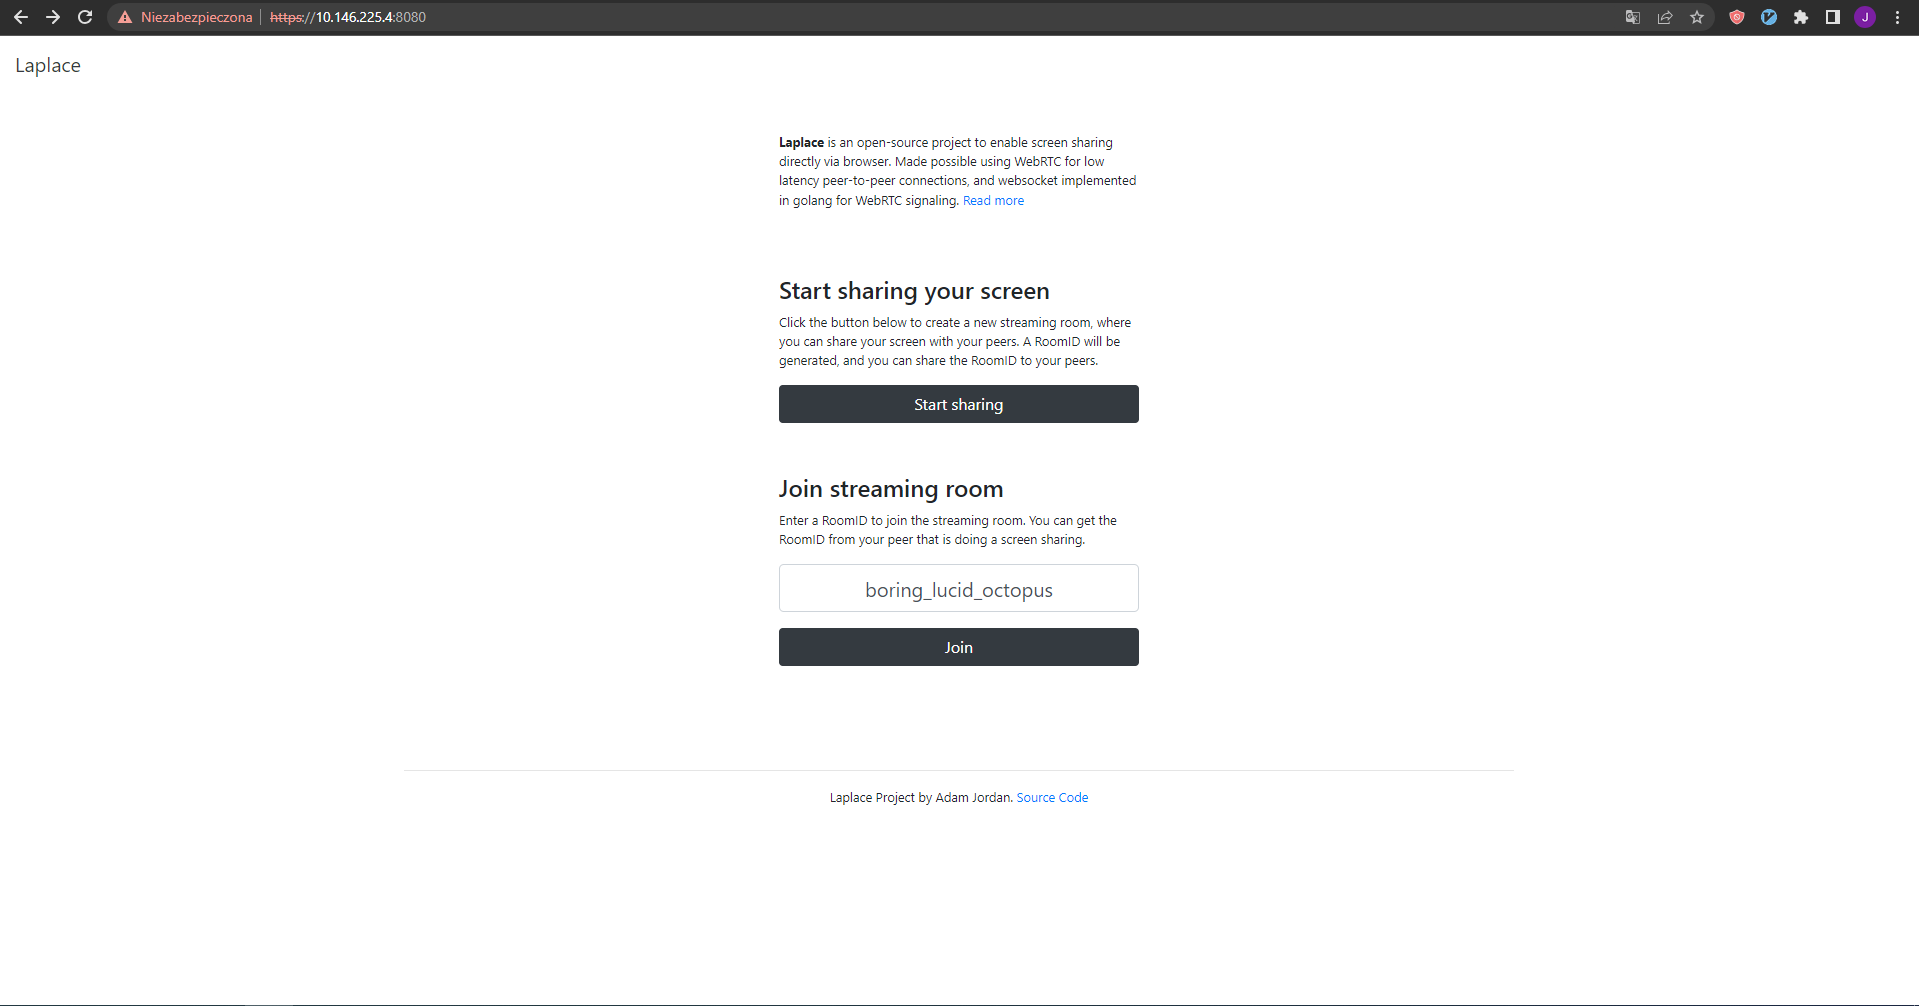
\includegraphics[width=1\textwidth]{glowna_strona.png}
        \end{figure}
        \begin{figure}[H]
            \caption{Zrzut ekranu strony udostępniania ekranu}
            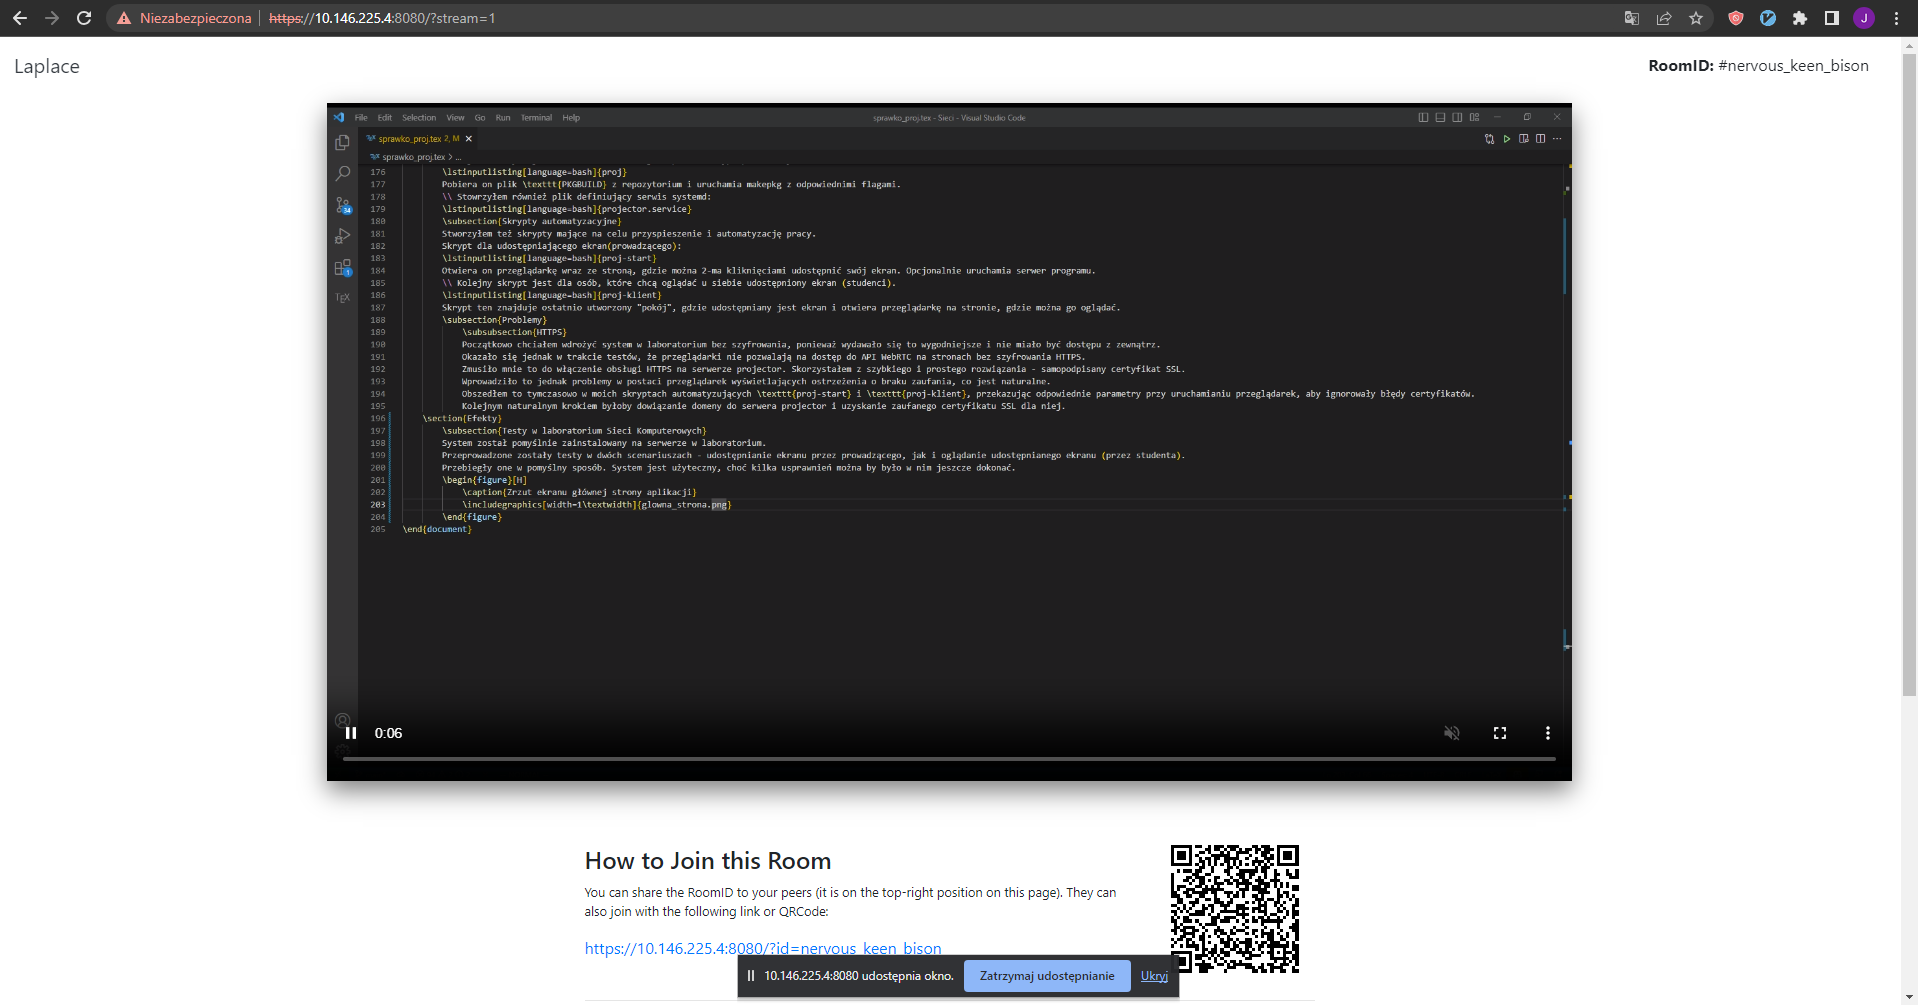
\includegraphics[width=1\textwidth]{strona_udostepniania.png}
        \end{figure}
        \subsection{Problemy i przyszłość}
            \subsubsection{HTTPS}
            Początkowo planowano wdrożyć system w laboratorium bez szyfrowania, ponieważ wydawało się to wygodniejsze i nie miało być dostępu z zewnątrz.
            Okazało się jednak w trakcie testów, że przeglądarki nie pozwalają na dostęp do API WebRTC na stronach bez szyfrowania HTTPS.
            Zmusiło to do włączenie obsługi HTTPS na serwerze projector. Skorzystano z szybkiego i prostego rozwiązania - samopodpisany certyfikat SSL.
            Wprowadziło to jednak problemy w postaci przeglądarek wyświetlających ostrzeżenia o braku zaufania, co jest naturalne. 
            Obchodzone jest to tymczasowo w moich skryptach automatyzujących \texttt{proj-start} i \texttt{proj-klient}, przekazując odpowiednie parametry przy uruchamianiu przeglądarek, aby ignorowały błędy certyfikatów.
            Kolejnym naturalnym krokiem byłoby dowiązanie domeny do serwera projector i uzyskanie zaufanego certyfikatu SSL dla niej. 
            \subsubsection{Protokoły okien}
            Podczas testów systemu w laboratorium okazało się, że poprawne działanie jest trudniejsze w przypadku używania nowoczesnego protokołu okien Wayland.
            Przeglądarki Chromium, Firefox nie dawały pełnych możliwości udostępnianie ekranu czy pojedynczych okien. 
            W przypadku przeglądarki Chromium nie uruchamiała się w ogóle w trybie Wayland, tylko korzystała z zapewniającego wsteczną kompatybilność protokołu XWayland.
            W pełni poprawną funkcjonalność udało się jedynie uzyskać wymuszając uruchomienie menedżera okien z protokołem X11 (Xorg).
            Jest to na pewno problem, który z czasem zostanie rozwiązany, ponieważ protokół Wayland jest przyszłością i jest dynamicznie rozwijany.
            \subsubsection{Konfiguracja wyświetlania strony}
            Interfejs użytkownika aplikacji można na pewno ulepszyć, tutaj kilka pomysłów: 
            \begin{itemize}
            \item Dodanie możliwości konfiguracji opcji WebRTC w utworzonym już pokoju - teraz można jedynie to robić przed jego utworzeniem.
            \item Lepsze możliwości zmiany rozmiaru okna oglądania udostępnianego ekranu - teraz można to robić jedynie przez zmianę rozmiaru okna przeglądarki i nie wykorzystuje dobrze ekranu.
            Przy trybie niepełnoekranowym występują problemy z rozdzielczością.
            \end{itemize}
    \section{Bibliografia i linki}
        \begin{thebibliography}{2}
        \bibitem{1} \url{https://github.com/jordus100/projector} - Repozytorium projektu
        \bibitem{2} \url{https://github.com/adamyordan/laplace} - Repozytorium oryginalnego systemu, na którym opiera się projekt
        \bibitem{3} \url{https://github.com/webrtc-for-the-curious/webrtc-for-the-curious} - Szczegółowy opis protokołu WebRTC
        \bibitem{4} \url{https://wiki.archlinux.org/title/PKGBUILD} % \\ \url{https://wiki.archlinux.org/title/makepkg} - Budowanie pakietów dla Arch Linux
        \bibitem{5} James Kurose, Keith Ross, "Computer networking a top-down approach", Pearson, 2017
        \bibitem{6} Kevin Fall, Richard Stevens, "TCP/IP Illustrated", Addison-Wesley, 20122
        \end{thebibliography}
\end{document}